% Compiler: pdfLaTeX
% =====================================================================
%  Mini-OpenClaw  --  Research poster  (Group 09, TU Wien, 194.211)
%  3 pages, each A3 LANDSCAPE (420mm x 297mm). Stack top->bottom to form
%  one tall poster (420mm wide x 891mm tall).
%  Page 1 = TOP, Page 2 = MIDDLE, Page 3 = BOTTOM.  Light theme.
%
%  Overleaf: Menu -> Compiler -> pdfLaTeX.  Upload optional images
%  tuwien-logo.png and ui-screenshot.png to the project root; if absent
%  labelled placeholders draw automatically.  Edit blocks marked
%  "EDIT EVAL DATA" to drop in real numbers.
% =====================================================================
\documentclass{article}

\usepackage[T1]{fontenc}
\usepackage[utf8]{inputenc}
\usepackage[paperwidth=420mm,paperheight=297mm,margin=10mm]{geometry}

% ---- Fonts: Fira Sans on Overleaf; graceful fallback to Helvetica ----
\IfFileExists{FiraSans.sty}{%
  \usepackage[sfdefault,scaled=1.02]{FiraSans}%
  \IfFileExists{FiraMono.sty}{\usepackage{FiraMono}}{}%
}{%
  \usepackage[scaled]{helvet}\renewcommand{\familydefault}{\sfdefault}%
}
\usepackage{microtype}
\usepackage{amssymb}
\usepackage{graphicx}
\usepackage{xcolor}
\usepackage{tikz}
\usepackage{pgfplots}\pgfplotsset{compat=1.18}
\usetikzlibrary{calc,positioning,arrows.meta,backgrounds,fit,shapes.geometric,shapes.misc}

% ---- Icons: fontawesome5 on Overleaf; harmless stubs as fallback -----
\IfFileExists{fontawesome5.sty}{\usepackage{fontawesome5}}{%
  \newcommand{\faProjectDiagram}{\textbullet}%
  \newcommand{\faDatabase}{\textbullet}%
  \newcommand{\faShieldAlt}{\textbullet}%
  \newcommand{\faLock}{\textbullet}%
  \newcommand{\faRobot}{\textbullet}%
  \newcommand{\faChartBar}{\textbullet}%
  \newcommand{\faLightbulb}{\textbullet}%
  \newcommand{\faFileAlt}{\textbullet}%
  \newcommand{\faAlignLeft}{\textbullet}%
  \newcommand{\faExclamationCircle}{\textbullet}%
  \newcommand{\faQuestionCircle}{\textbullet}%
  \newcommand{\faBolt}{\textbullet}%
  \newcommand{\faCheckCircle}{\textbullet}%
  \newcommand{\faExclamationTriangle}{\textbullet}%
  \newcommand{\faTimesCircle}{\textbullet}%
  \newcommand{\faCheck}{\textbullet}%
  \newcommand{\faGithub}{\textbullet}%
  \newcommand{\faClock}{\textbullet}%
  \newcommand{\faSitemap}{\textbullet}%
  \newcommand{\faTerminal}{\textbullet}%
  \newcommand{\faLayerGroup}{\textbullet}%
  \newcommand{\faPuzzlePiece}{\textbullet}%
  \newcommand{\faServer}{\textbullet}%
  \newcommand{\faSyncAlt}{\textbullet}%
  \newcommand{\faArrowRight}{$\rightarrow$}%
  \newcommand{\faCogs}{\textbullet}%
}

% --------------------------- COLOUR SYSTEM ---------------------------
\definecolor{tublue}{HTML}{0063A6}   % TU Wien blue (primary)
\definecolor{tblued}{HTML}{004E83}   % darker blue
\definecolor{ink}{HTML}{0B1F3A}      % headings
\definecolor{inkt}{HTML}{223247}     % body text
\definecolor{slate}{HTML}{5C6B7A}    % secondary text
\definecolor{line}{HTML}{DCE2E9}     % hairlines
\definecolor{paper}{HTML}{F5F7FA}    % page background (light)
\definecolor{panel}{HTML}{ECF1F6}    % faint panel tint
\definecolor{teal}{HTML}{0E8F89}     % accent (readable on light)
\definecolor{amber}{HTML}{D98000}    % approval
\definecolor{coral}{HTML}{D9494E}    % forbidden / emphasis
\definecolor{safe}{HTML}{1E9B68}     % safe / success
% chart series
\definecolor{barbase}{HTML}{A7B3BF}
\definecolor{bartwo}{HTML}{2E86C1}
\definecolor{barfull}{HTML}{0E8F89}

\setlength{\parindent}{0pt}
\pagestyle{empty}

% --------------------------- TYPE HELPERS ----------------------------
\newcommand{\HeroTitle}{\fontsize{52}{54}\selectfont\bfseries}
\newcommand{\Tag}{\fontsize{18}{22}\selectfont}
\newcommand{\PanelTitle}{\fontsize{30}{32}\selectfont\bfseries}
\newcommand{\Kick}{\fontsize{12}{14}\selectfont\bfseries}
\newcommand{\SecHead}{\fontsize{15}{18}\selectfont\bfseries}
\newcommand{\Body}{\fontsize{11}{15}\selectfont}
\newcommand{\BodyS}{\fontsize{10}{13.5}\selectfont}
\newcommand{\Mini}{\fontsize{8.6}{10.8}\selectfont}
\newcommand{\StatNum}{\fontsize{36}{36}\selectfont\bfseries}
\newcommand{\BodyL}{\fontsize{12.5}{17}\selectfont}
% hanging-indent bullet: wrapped lines align under the text, not the bullet
\newlength{\bsp}\setlength{\bsp}{2.8mm}
\newcommand{\bitem}[1]{\hangindent=4.4mm\hangafter=1\noindent\makebox[4.4mm][l]{$\bullet$}#1\par\vspace{\bsp}}

% --------------------------- TIKZ STYLES -----------------------------
\tikzset{
  >={Stealth[length=2.6mm,width=2.0mm]},
  card/.style={rounded corners=2.6mm, draw=line, line width=0.4mm, fill=white},
  tintcard/.style={rounded corners=2.6mm, draw=line, line width=0.4mm, fill=panel},
  pill/.style={rounded corners=2mm, inner xsep=2.6mm, inner ysep=1.3mm, font=\BodyS\bfseries},
  minipill/.style={rounded corners=1.8mm, inner xsep=2mm, inner ysep=1mm, font=\Mini\bfseries},
  % diagram blocks
  bprime/.style={rounded corners=2mm, fill=tublue, draw=tblued, line width=0.3mm, text=white,
                 align=center, font=\BodyS\bfseries, inner sep=1.6mm},
  bio/.style={rounded corners=2mm, fill=teal, text=white, align=center, font=\BodyS\bfseries, inner sep=1.6mm},
  bsec/.style={rounded corners=2mm, fill=white, draw=tublue, line width=0.45mm, text=tublue,
               align=center, font=\BodyS\bfseries, inner sep=1.6mm},
  bfin/.style={rounded corners=2mm, fill=safe, text=white, align=center, font=\BodyS\bfseries, inner sep=1.6mm},
  flow/.style={-{Stealth[length=2.8mm]}, line width=0.6mm, draw=ink},
  flowt/.style={-{Stealth[length=2.8mm]}, line width=0.55mm, draw=teal},
  lab/.style={fill=white, inner sep=0.6mm, font=\Mini, text=slate},
  labt/.style={fill=white, inner sep=0.6mm, font=\Mini\bfseries, text=teal},
}

% --------------------------- LONG TEXT -------------------------------
\def\abstractText{%
Mini-OpenClaw is a local-first AI agent that turns plain-language requests
into safe, auditable actions on your own machine. Ask it to \textbf{organise and
search files}, \textbf{read and edit documents}, \textbf{run shell commands},
\textbf{fetch live web data}, \textbf{remember facts across sessions},
\textbf{schedule recurring jobs}, or \textbf{delegate multi-step tasks} to
sub-agents --- each behind a real-time approval gate and a full audit trail.\\[4mm]
Under the hood a hybrid \textbf{Plan\,$\rightarrow$\,ReAct\,$\rightarrow$\,Replan}
loop reasons step by step and revises its plan when an action fails, while a
policy engine classifies every call as \emph{safe}, \emph{approval-required}, or
\emph{forbidden} before it runs. The result is a small but complete agent ---
autonomous enough to be useful, constrained enough to trust --- running locally
through swappable Anthropic, Gemini, or Ollama providers.

}

\def\problemText{%
General-purpose LLM agents are powerful but hard to trust: they take
consequential actions --- writing files, running shell commands, fetching the
web --- with little visibility into what was decided or why, and most depend
on remote APIs that cost money and leak data. We wanted an agent we could read
end to end, run offline at zero cost, and inspect after every run. The
challenge was to stay autonomous enough to finish multi-step tasks while
making each tool call explicit, permission-checked, and reversible.

}

% =====================================================================
\begin{document}

% #####################################################################
% #  PANEL 1 (TOP)  --  Identity & Framing                            #
% #####################################################################
\thispagestyle{empty}%
\begin{tikzpicture}[remember picture, overlay]
  \coordinate (NW) at (current page.north west);
  \fill[paper] (current page.south west) rectangle (current page.north east);
  % header bar
  \fill[tublue] (NW) rectangle ($(NW)+(420mm,-26mm)$);
  \fill[teal]   ($(NW)+(0,-26mm)$) rectangle ($(NW)+(420mm,-27.4mm)$);

  % header: logo on a white plate (TU Wien logo reads poorly directly on blue) ---
  \node[anchor=north west, fill=white, rounded corners=2.2mm, inner sep=2.4mm] at ($(NW)+(14mm,-2.6mm)$){%
    \IfFileExists{tuwien-logo.png}{\includegraphics[height=16.5mm]{tuwien-logo.png}}{%
      \tikz{\node[rounded corners=1.4mm, draw=tublue, dash pattern=on 1.4mm off 1.2mm,
                  line width=0.3mm, text=tublue, align=center, minimum height=14.5mm,
                  inner xsep=3mm, font=\Mini]{[\,TU Wien logo\,]\\ \textit{supply tuwien-logo.png}};}}};
  % header: course / version (right, trimmed)
  \node[anchor=north east, align=right, text=white] at ($(NW)+(404mm,-6mm)$){%
    {\BodyS\bfseries 194.211 Applied Generative AI \& LLM-based Systems}\\[1mm]
    {\Mini v0.1.0 \ \ $\cdot$\ \ status: in-progress}};

  % logo mark + title (left)
  \node[anchor=north west, minimum size=22mm, rounded corners=4mm, fill=tublue] (mk)
        at ($(NW)+(16mm,-40mm)$) {};
  \node at (mk.center) {\fontsize{18}{18}\selectfont\bfseries\ttfamily\color{white}$\rangle$\_};
  \node[anchor=west, text=ink] (ttl) at ($(mk.east)+(6mm,1.5mm)$) {\HeroTitle Mini\textcolor{tublue}{-}OpenClaw};
  \fill[teal] ($(NW)+(44mm,-65mm)$) rectangle ($(NW)+(196mm,-66.6mm)$);
  \node[anchor=north west, text=tublue] at ($(NW)+(44mm,-68mm)$){\Tag Local-first AI agents you can actually trust.};

  % group + members (RIGHT of the title)
  \node[anchor=north east, card, text width=176mm, minimum height=44mm, inner sep=4.5mm, align=left]
       (gcard) at ($(NW)+(404mm,-34mm)$){};
  \node[pill, fill=tublue, text=white, anchor=north west] (grp) at ($(gcard.north west)+(4.5mm,-4.2mm)$){GROUP 09};
  \node[anchor=west, text=slate] at ($(grp.east)+(3mm,0)$){\BodyS Applied Generative AI --- course project};
  \foreach \i/\j/\nm/\id in {%
      0/0/{Held Johannes}/{11705340}, 0/1/{Ibrahim Ahmad}/{11826186},
      1/0/{Ibrar Muhammad}/{12350094}, 1/1/{Bourbigua Manal}/{12347522}}{
    \node[anchor=north west, text=ink, align=left]
      at ($(gcard.north west)+(5mm+\j*84mm,-17mm-\i*11mm)$){%
        {\BodyS\bfseries \nm}\\[0.4mm]{\Mini\color{slate}\#\,\id}};
  }

  % Abstract card (left) -- taller, narrower, gutter
  \node[anchor=north west, card, text width=168mm, minimum height=95mm, inner sep=5.5mm, align=left]
       (abs) at ($(NW)+(16mm,-92mm)$){};
  \node[anchor=north west, text=tublue] at ($(abs.north west)+(5.5mm,-5.5mm)$){\SecHead \faAlignLeft~~Abstract};
  \node[anchor=north west, text=inkt, text width=157mm, align=left] at ($(abs.north west)+(5.5mm,-15mm)$){\BodyL\abstractText};

  % Problem card (right) -- gutter between
  \node[anchor=north west, card, text width=192mm, minimum height=95mm, inner sep=5.5mm, align=left]
       (prob) at ($(NW)+(196mm,-92mm)$){};
  \node[anchor=north west, text=coral] at ($(prob.north west)+(5.5mm,-5.5mm)$){\SecHead \faExclamationCircle~~The problem / initial situation};
  \node[anchor=north west, text=inkt, text width=181mm, align=left] at ($(prob.north west)+(5.5mm,-15mm)$){\BodyL\problemText};

  % What it delivers -- four pillars
  \node[anchor=north west, text=ink] at ($(NW)+(16mm,-193mm)$){\SecHead What it delivers};
  \fill[teal] ($(NW)+(16mm,-202mm)$) rectangle ($(NW)+(70mm,-203.2mm)$);
  \foreach \i/\ic/\cl/\ti/\bd in {%
      0/{\faSitemap}/{tublue}/{Intent $\rightarrow$ tool routing}/{A planner turns plain language into a validated JSON plan. The LLM proposes; code decides.\\},
      1/{\faLayerGroup}/{teal}/{Auditable memory}/{Five memory layers (vector + keyword) and an append-only audit log --- every decision inspectable.\\},
      2/{\faPuzzlePiece}/{amber}/{Extensible skills}/{Manifest-driven registry: add a tool by adding a module --- no core-loop changes.\\},
      3/{\faLock}/{coral}/{Safe execution}/{A policy engine gates every action as safe, approval-required, or forbidden before it runs.\\}}{
    \node[anchor=north west, card, text width=81mm, minimum height=48mm, inner sep=5mm, align=left]
         (pil\i) at ($(NW)+(16mm+\i*97mm,-207mm)$){};
    \node[anchor=north west, text=\cl] at ($(pil\i.north west)+(5mm,-4.6mm)$){\fontsize{16}{16}\selectfont\ic};
    \node[anchor=north west, text=ink, text width=71mm, align=left] at ($(pil\i.north west)+(15mm,-4.4mm)$){\SecHead \ti};
    \node[anchor=north west, text=inkt, text width=71mm, align=left] at ($(pil\i.north west)+(5mm,-16mm)$){\BodyS \bd};
  }

  % by the numbers -- meaningful three (left) + tech stack (right)
  \node[anchor=north west, tintcard, minimum width=388mm, minimum height=35mm]
       (num) at ($(NW)+(16mm,-259mm)$){};
  \foreach \i/\n/\l in {0/{13 + MCP}/{tools}, 1/{3}/{LLM providers tested}, 2/{5}/{memory layers}}{
    \node[anchor=north, text=tublue] at ($(NW)+(58mm+\i*68mm,-264mm)$){\StatNum \n};
    \node[anchor=north, text=slate] at ($(NW)+(58mm+\i*68mm,-281mm)$){\BodyS \l};
  }
  \draw[line,line width=0.3mm] ($(NW)+(248mm,-265mm)$)--($(NW)+(248mm,-288mm)$);
  \node[anchor=north, text=inkt, text width=140mm, align=center] at ($(NW)+(330mm,-264mm)$){%
    {\Mini\bfseries\color{ink}TECH STACK}\\[2mm]
    {\BodyS Backend: FastAPI $\cdot$ SQLite}\\[1.2mm]
    {\BodyS Frontend: React + TypeScript (Vite) $\cdot$ SSE}};
\end{tikzpicture}%
\null\clearpage

% #####################################################################
% #  PANEL 2 (MIDDLE)  --  Approach                                   #
% #####################################################################
\thispagestyle{empty}%
\begin{tikzpicture}[remember picture, overlay]
  \coordinate (NW) at (current page.north west);
  \fill[paper] (current page.south west) rectangle (current page.north east);
  \fill[tublue] (NW) rectangle ($(NW)+(420mm,-2mm)$);          % top seam
  \fill[teal]   ($(NW)+(0,-295mm)$) rectangle ($(NW)+(420mm,-297mm)$); % bottom seam

  % title
  \node[anchor=north west, text=tublue] at ($(NW)+(16mm,-10mm)$){\Kick HOW IT WORKS};
  \node[anchor=north west, text=ink] at ($(NW)+(16mm,-14mm)$){\PanelTitle \faProjectDiagram~~Approach};
  % intro text
  \node[anchor=north west, text=inkt, text width=388mm, align=left] at ($(NW)+(16mm,-30mm)$){%
    \Body Every request runs as one auditable loop. The \textbf{planner} proposes a single next step; the
    \textbf{policy engine} classifies it as safe, approval-required, or forbidden; the \textbf{executor} runs it; and the
    \textbf{observation} feeds back so the planner can continue, adapt, or replan. When the goal is met the loop returns a
    \textbf{final answer}. Around it, \textcolor{tublue}{\textbf{memory}} supplies context, the
    \textcolor{tublue}{\textbf{audit log}} records every decision, and \textcolor{tublue}{\textbf{SSE}} streams progress to the UI.};

  % ---- BLOCK DIAGRAM (clean, left-to-right) ----
  \node[anchor=north west, card, minimum width=388mm, minimum height=124mm] (dia) at ($(NW)+(16mm,-44mm)$){};
  \node[anchor=center] at (dia.center){%
  \begin{tikzpicture}[x=1mm,y=1mm]
    % orchestrator header strip
    \fill[tublue, rounded corners=1.6mm] (0,96) rectangle (360,104);
    \node[text=white, font=\BodyS\bfseries] at (180,100){ORCHESTRATOR \;\textmd{$\cdot$\; owns the run lifecycle --- the LLM proposes, code decides}};
    % lane blocks
    \node[bio,    minimum width=38mm, minimum height=16mm] (usr) at (28,64) {User\\ request};
    \node[bprime, minimum width=44mm, minimum height=20mm] (pla) at (96,64) {PLANNER};
    \node[bprime, minimum width=44mm, minimum height=20mm] (pol) at (166,64){POLICY\\ ENGINE};
    \node[bprime, minimum width=44mm, minimum height=20mm] (exe) at (236,64){EXECUTOR};
    \node[bsec,   minimum width=44mm, minimum height=20mm] (obs) at (306,64){OBSERVATION};
    \node[bfin,   minimum width=44mm, minimum height=16mm] (fin) at (306,30){FINAL ANSWER};
    % straight lane arrows
    \draw[flow] (usr) -- (pla);
    \draw[flow] (pla) -- node[lab,above=0.4mm]{propose step} (pol);
    \draw[flow] (pol) -- node[lab,above=0.4mm]{verdict} (exe);
    \draw[flow] (exe) -- node[lab,above=0.4mm]{run tool} (obs);
    % observation -> final (done) and feedback loop (re-plan)
    \draw[flow] (obs) -- node[lab,right=0.6mm,pos=0.5]{goals met} (fin);
    \draw[flowt] (obs.north) .. controls (306,90) and (96,90) ..
        node[labt,pos=0.5]{not done $\rightarrow$ observe \& re-plan (the ReAct loop)} (pla.north);
    % policy verdict pills (under policy)
    \node[minipill, fill=safe,  text=white, anchor=north] at (166,50){safe $\rightarrow$ auto};
    \node[minipill, fill=amber, text=white, anchor=north] at (166,43){approval $\rightarrow$ user};
    \node[minipill, fill=coral, text=white, anchor=north] at (166,36){forbidden $\rightarrow$ block};
    % around-the-loop chips
    \node[anchor=west, text=slate, font=\Mini\bfseries] at (0,16){AROUND THE LOOP};
    \node[minipill, draw=tublue, text=tublue, anchor=west] at (0,9) {\faLayerGroup\ Memory $\rightarrow$ planner context};
    \node[minipill, draw=tublue, text=tublue, anchor=west] at (122,9){\faAlignLeft\ Audit $\leftarrow$ every step};
    \node[minipill, draw=tublue, text=tublue, anchor=west] at (236,9){\faBolt\ SSE $\rightarrow$ live UI};
  \end{tikzpicture}};

  % ---- support row : three cards ----
  % Card A: five-layer memory
  \node[anchor=north west, card, text width=120mm, minimum height=92mm, inner sep=5mm, align=left]
       (cA) at ($(NW)+(16mm,-176mm)$){};
  \node[anchor=north west, text=tublue] at ($(cA.north west)+(5mm,-5mm)$){\SecHead \faLayerGroup~~Five-layer memory};
  \node[anchor=north west] at ($(cA.north west)+(5mm,-15mm)$){%
    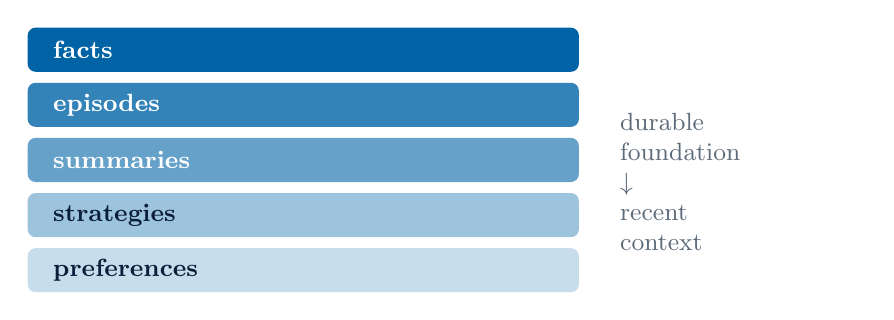
\begin{tikzpicture}[x=1mm,y=1mm]
      \foreach \i/\nm/\sh/\tc in {0/facts/100/white, 1/episodes/80/white, 2/summaries/60/white,
                                  3/strategies/38/ink, 4/preferences/22/ink}{
        \fill[tublue!\sh!white, rounded corners=1mm] (0,32-\i*7) rectangle (70,32-\i*7+5.6);
        \node[anchor=west, text=\tc, font=\Mini\bfseries] at (2,32-\i*7+2.8){\nm};
      }
      \node[anchor=west, text=slate, text width=30mm, font=\Mini, align=left] at (74,18)
        {durable\\ foundation\\ $\downarrow$\\ recent\\ context};
    \end{tikzpicture}};
  \node[anchor=north west, text width=110mm, align=left] at ($(cA.north west)+(5mm,-54mm)$){%
    {\BodyS\color{inkt}\textbf{Hybrid retrieval} blends \textcolor{tublue}{70\% vector} (local \texttt{all-MiniLM-L6-v2}, \$0) + \textcolor{tublue}{30\% keyword}, injected into the planner each call.}\\[7mm]
    {\BodyS\color{inkt}\textbf{Agent Dreams} consolidate runs into proposed strategies under \emph{propose $\rightarrow$ review $\rightarrow$ approve} --- never acting on inferred knowledge without consent.}};

  % Card B: safe by design
  \node[anchor=north west, card, text width=120mm, minimum height=92mm, inner sep=5mm, align=left]
       (cB) at ($(NW)+(150mm,-176mm)$){};
  \node[anchor=north west, text=coral] at ($(cB.north west)+(5mm,-5mm)$){\SecHead \faLock~~Safe by design};
  \node[anchor=north west] at ($(cB.north west)+(5mm,-15mm)$){%
    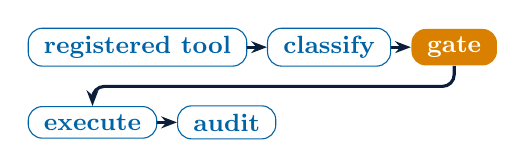
\begin{tikzpicture}[x=1mm,y=1mm, font=\Mini\bfseries]
      \node[minipill, draw=tublue, text=tublue] (s1) {registered tool};
      \node[minipill, draw=tublue, text=tublue, right=2.5mm of s1] (s2) {classify};
      \node[minipill, fill=amber, text=white, right=2.5mm of s2] (s3) {gate};
      \node[minipill, draw=tublue, text=tublue, below=5mm of s1.south west, anchor=north west] (s4) {execute};
      \node[minipill, draw=tublue, text=tublue, right=2.5mm of s4] (s5) {audit};
      \draw[-{Stealth[length=2mm]},draw=ink,line width=0.4mm] (s1)--(s2);
      \draw[-{Stealth[length=2mm]},draw=ink,line width=0.4mm] (s2)--(s3);
      \draw[-{Stealth[length=2mm]},draw=ink,line width=0.4mm,rounded corners=1.5mm] (s3.south) -- ++(0,-2.6mm) -| (s4.north);
      \draw[-{Stealth[length=2mm]},draw=ink,line width=0.4mm] (s4)--(s5);
    \end{tikzpicture}};
  \node[anchor=north west] at ($(cB.north west)+(5mm,-42mm)$){%
    
\begin{tikzpicture}[x=1mm,y=1mm]
      \node[minipill, fill=safe,  text=white] (a){\faCheckCircle\ safe};
      \node[minipill, fill=amber, text=white, right=2.5mm of a] (b){\faExclamationTriangle\ approval};
      \node[minipill, fill=coral, text=white, right=2.5mm of b] (c){\faTimesCircle\ forbidden};
    \end{tikzpicture}};
  \node[anchor=north west, text width=110mm, align=left] at ($(cB.north west)+(5mm,-56mm)$){%
    {\BodyS\color{inkt}Only registered tools with valid JSON schemas run. The policy engine enforces workspace path limits, shell allow-lists, and prompt-injection checks.}\\[7mm]
    {\BodyS\color{inkt}Risky writes, shell, web-fetch, and delegation need explicit approval --- and \textcolor{tublue}{approval is invalidated if the payload changes}.}};

  % Card C: providers + tools
  \node[anchor=north west, card, text width=120mm, minimum height=92mm, inner sep=5mm, align=left]
       (cC) at ($(NW)+(284mm,-176mm)$){};
  \node[anchor=north west, text=tublue] at ($(cC.north west)+(5mm,-5mm)$){\SecHead \faServer~~Providers \& tools};
  \node[anchor=north west] at ($(cC.north west)+(5mm,-15mm)$){%
    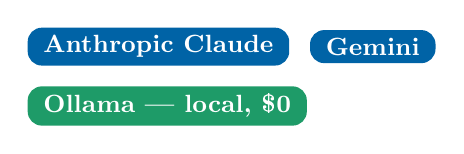
\begin{tikzpicture}[x=1mm,y=1mm, font=\Mini\bfseries]
      \node[minipill, fill=tublue, text=white] (p1){Anthropic Claude};
      \node[minipill, fill=tublue, text=white, right=2.5mm of p1] (p2){Gemini};
      \node[minipill, fill=safe, text=white, below=2.5mm of p1.south west, anchor=north west] (p3){Ollama --- local, \$0};
    \end{tikzpicture}};
  \node[anchor=north west, text width=110mm, align=left] at ($(cC.north west)+(5mm,-31mm)$){%
    {\Mini\bfseries\color{ink}13 TOOLS}\ {\Mini\color{slate}($\ast$ = approval-gated)}\\[1.6mm]
    {\Mini\color{inkt}\texttt{list\_files} $\cdot$ \texttt{read\_file} $\cdot$ \texttt{write\_file}$\ast$ $\cdot$ \texttt{search\_in\_files} $\cdot$ \texttt{run\_shell\_safe}$\ast$ $\cdot$ \texttt{remember\_fact} $\cdot$ \texttt{search\_memory} $\cdot$ \texttt{delegate\_task}$\ast$ $\cdot$ \texttt{fetch\_url}$\ast$ $\cdot$ \texttt{schedule\_task} $\cdot$ \texttt{get\_datetime} $\cdot$ \texttt{calculator} $\cdot$ \texttt{system\_info} \\ \vspace{1mm} $+$ \textbf{(explain\_run} $\cdot$ \textbf{mcp\_tool$\ast$)}}};
  \node[anchor=north west, text width=110mm, align=left] at ($(cC.north west)+(5mm,-58mm)$){%
    {\BodyS\color{inkt}A manifest declares each tool's schema, risk level, and approval flag. The registry discovers tools at startup --- the planner only sees registered tools, and adding one needs no core changes.}\\[5mm]
    {\BodyS\color{inkt}\textbf{MCP interop}: act as \emph{client} (consume external tools) or \emph{server} (expose tools to Claude Desktop and others). Default off; proxy tools gated at HIGH risk.}};
\end{tikzpicture}%
\null\clearpage

% #####################################################################
% #  PANEL 3 (BOTTOM)  --  Results & Reflection                       #
% #####################################################################
\thispagestyle{empty}%
\begin{tikzpicture}[remember picture, overlay]
  \coordinate (NW) at (current page.north west);
  \fill[paper] (current page.south west) rectangle (current page.north east);
  \fill[tublue] (NW) rectangle ($(NW)+(420mm,-2mm)$);          % top seam

  % title
  \node[anchor=north west, text=tublue] at ($(NW)+(16mm,-10mm)$){\Kick WHAT IT DOES TODAY};
  \node[anchor=north west, text=ink] at ($(NW)+(16mm,-14mm)$){\PanelTitle \faChartBar~~Results \& Reflection};

  % ---- Row 1: screenshot (left) + capability matrix (right) ----
  \node[anchor=north west, card, minimum width=216mm, minimum height=100mm] (shot) at ($(NW)+(16mm,-32mm)$){};
  \fill[ink, rounded corners=2.6mm] ($(shot.north west)$) rectangle ($(shot.north east)+(0,-7mm)$);
  \fill[ink] ($(shot.north west)+(0,-3.5mm)$) rectangle ($(shot.north east)+(0,-7mm)$);
  \foreach \k in {0,1,2}{\fill[white] ($(shot.north west)+(4mm+\k*4mm,-3.5mm)$) circle (1mm);}
  \node[anchor=west, text=white, font=\Mini] at ($(shot.north west)+(16mm,-3.5mm)$){Mini-OpenClaw \ $\cdot$\ localhost:5173};
  \node at ($(shot.center)+(0,-3mm)$){%
    \IfFileExists{ui-screenshot.png}{\includegraphics[width=205mm]{ui-screenshot.png}}{%
      \tikz{\node[rounded corners=1.6mm, draw=slate, dash pattern=on 1.6mm off 1.4mm, line width=0.3mm,
                  text=slate, align=center, minimum width=196mm, minimum height=80mm, font=\BodyS]
                  {[\ UI screenshot\ ]\\[1mm]\textit{supply ui-screenshot.png}};}}};

  \node[anchor=north west, card, text width=160mm, minimum height=100mm, inner sep=5mm, align=left]
       (cap) at ($(NW)+(244mm,-32mm)$){};
  \node[anchor=north west, text=ink] at ($(cap.north west)+(5mm,-5mm)$){\SecHead Capability success (\%)};
  \node[anchor=north] at ($(cap.north)+(0,-13mm)$){%
    \begin{tikzpicture}[x=1mm,y=1mm, font=\Mini]
      % column headers
      \foreach \c/\cn in {0/Baseline, 1/{Plan+ReAct}, 2/Full}{
        \node[anchor=south, text=ink, font=\Mini\bfseries] at (44+\c*32+16,4){\cn};}
      % EDIT EVAL DATA: rows = capability; values = Baseline / ReAct / Full
      \foreach \r/\nm/\a/\b/\d in {%
          0/recall/54.2/95.8/100, 
          1/search/41.7/75/75, 
          2/completeness/100/100/100,
          3/multi-step/27.8/94.4/100, 
          4/recovery/0/80/100, 
          5/cross-file/100/100/100,
          6/memory/100/100/100, 
          7/delegation/50/100/100}{
        \node[anchor=east, text=inkt] at (42,-\r*9-3){\nm};
        \foreach \c/\v in {0/\a, 1/\b, 2/\d}{
          \fill[tublue!\v!white, rounded corners=0.8mm] (44+\c*32,-\r*9-6.3) rectangle (44+\c*32+30,-\r*9+0.3);
          \pgfmathparse{\v<58?"ink":"white"}\edef\tc{\pgfmathresult}
          \node[anchor=center, text=\tc, font=\Mini\bfseries] at (44+\c*32+15,-\r*9-3){\v};}
      }
    \end{tikzpicture}};

  % ---- Row 2: three charts (full width) ----
  \node[anchor=north west, text=ink] at ($(NW)+(16mm,-136mm)$){\SecHead Where the pipeline earns its cost};
  \node[anchor=north west, text=inkt, text width=388mm, align=left] at ($(NW)+(16mm,-143mm)$){%
    \BodyS \textbf{Method:} 14 deterministic tasks across 8 capability categories, run in a sandboxed fixture workspace and
    scored by deterministic verifiers (file contents, keyword presence, numeric answers) --- no LLM-as-judge. Across the suite
    (Baseline plan-and-execute vs.\ Plan+ReAct vs.\ the Full hybrid), the full loop spends more tool calls and money per run
    but wins clearly on \textbf{completeness}, \textbf{recovery}, and \textbf{multi-step} tasks.};

 
% chart 1: success rate
  \node[anchor=north west] at ($(NW)+(28mm,-156mm)$){%
    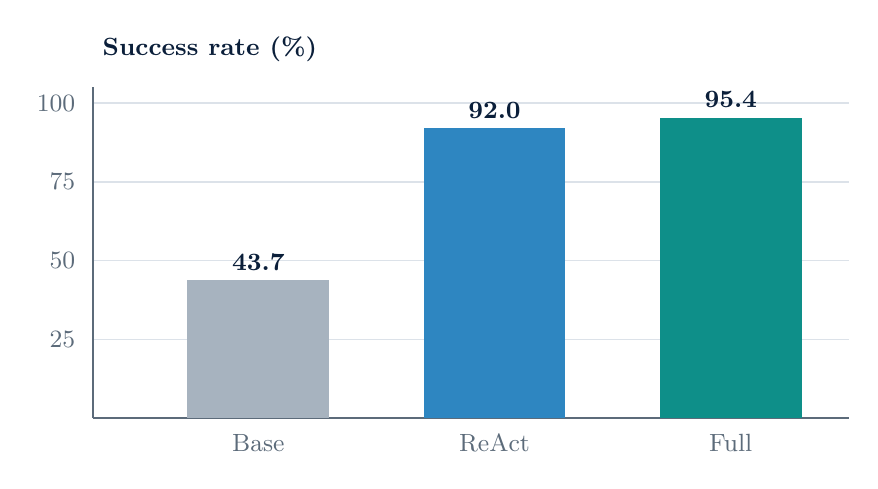
\begin{tikzpicture}[x=1mm,y=1mm, font=\Mini]
      \node[anchor=south west, text=ink, font=\Mini\bfseries] at (0,44){Success rate (\%)};
      \foreach \g in {25,50,75,100}{\draw[line,line width=0.2mm](0,\g*0.40)--(96,\g*0.40);
        \node[anchor=east,text=slate] at (-1,\g*0.40){\g};}
      \draw[slate,line width=0.3mm](0,0)--(0,42); \draw[slate,line width=0.3mm](0,0)--(96,0);
      % EDIT EVAL DATA
      \foreach \x/\v/\c/\nm in {12/43.7/barbase/Base, 42/92.0/bartwo/ReAct, 72/95.4/barfull/Full}{
        \fill[\c] (\x,0) rectangle (\x+18,\v*0.40);
        \node[anchor=south,text=ink,font=\Mini\bfseries] at (\x+9,\v*0.40){\v};
        \node[anchor=north,text=slate] at (\x+9,-0.8){\nm};}
    \end{tikzpicture}};
  % chart 2: avg tool calls
\node[anchor=north west] at ($(NW)+(160mm,-156mm)$){%
    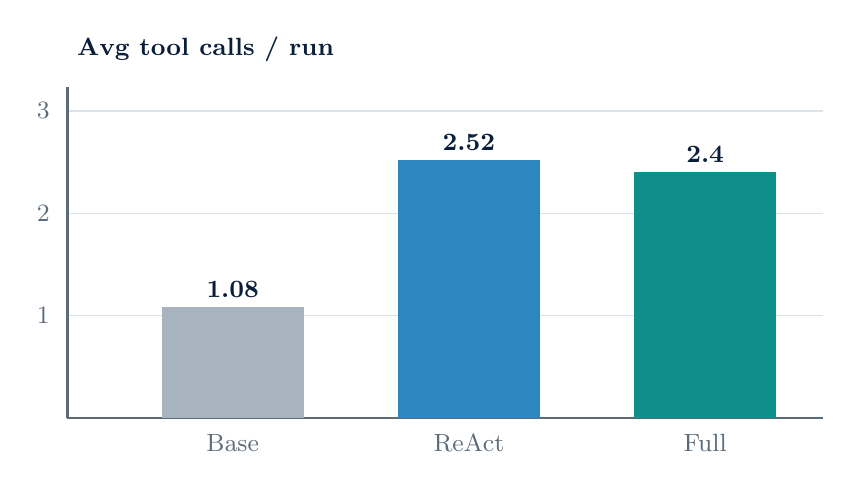
\begin{tikzpicture}[x=1mm,y=1mm, font=\Mini]
      \node[anchor=south west, text=ink, font=\Mini\bfseries] at (0,44){Avg tool calls / run};
      \foreach \g in {1,2,3}{\draw[line,line width=0.2mm](0,\g*13.0)--(96,\g*13.0);
        \node[anchor=east,text=slate] at (-1,\g*13.0){\g};}
      \draw[slate,line width=0.3mm](0,0)--(0,42); \draw[slate,line width=0.3mm](0,0)--(96,0);
      % EDIT EVAL DATA
      \foreach \x/\v/\c/\nm in {12/1.08/barbase/Base, 42/2.52/bartwo/ReAct, 72/2.4/barfull/Full}{
        \fill[\c] (\x,0) rectangle (\x+18,\v*13.0);
        \node[anchor=south,text=ink,font=\Mini\bfseries] at (\x+9,\v*13.0){\v};
        \node[anchor=north,text=slate] at (\x+9,-0.8){\nm};}
    \end{tikzpicture}};
  % chart 3: cost vs success scatter
  \node[anchor=north west] at ($(NW)+(292mm,-156mm)$){%
    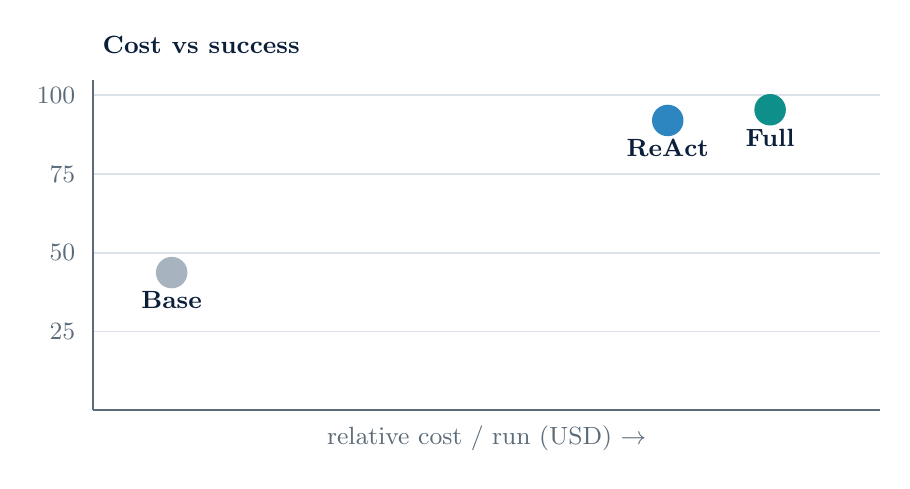
\begin{tikzpicture}[x=1mm,y=1mm, font=\Mini]
      \node[anchor=south west, text=ink, font=\Mini\bfseries] at (0,44){Cost vs success}; %
      \foreach \g in {25,50,75,100}{\draw[line,line width=0.2mm](0,\g*0.40)--(100,\g*0.40);
        \node[anchor=east,text=slate] at (-1,\g*0.40){\g};}
      \draw[slate,line width=0.3mm](0,0)--(0,42); \draw[slate,line width=0.3mm](0,0)--(100,0);
      % EDIT EVAL DATA: cx = cost position
      \foreach \cx/\v/\c/\nm/\an in {10/43.7/barbase/Base/below, 73/92.0/bartwo/ReAct/below, 86/95.4/barfull/Full/below}{
        \fill[\c] (\cx,\v*0.40) circle (2mm);
        \node[text=ink,font=\Mini\bfseries,\an=1.2mm] at (\cx,\v*0.40){\nm};}
      \node[anchor=north,text=slate] at (50,-0.8){relative cost / run (USD) $\rightarrow$};
    \end{tikzpicture}};

  % ---- Row 3: three learnings cards (top-aligned) ----
  \foreach \i/\cl/\ic/\ti in {%
      0/{safe}/{\faCheckCircle}/{What worked well},
      1/{amber}/{\faExclamationTriangle}/{Challenges},
      2/{tublue}/{\faLightbulb}/{Further work}}{
    \node[anchor=north west, card, text width=120mm, minimum height=70mm, inner sep=5mm, align=left]
         (lc\i) at ($(NW)+(16mm+\i*134mm,-212mm)$){};
    \node[anchor=north west, text=\cl] at ($(lc\i.north west)+(5mm,-5mm)$){\SecHead \ic~~\ti};
  }
  % worked
  \node[anchor=north west, text width=110mm, text=inkt, align=left] at ($(lc0.north west)+(5mm,-15mm)$){%
    \BodyS\setlength{\bsp}{4mm}%
    \bitem{Separating planning / policy / execution / memory / logging made the agent debuggable.}
    \bitem{Policy engine + approval gates gave safety without crippling capability.}
    \bitem{The hybrid loop improved completeness and recovery over a plain plan-and-execute baseline.}
    \bitem{Local embeddings give useful semantic memory at no extra cost (\$0).}};
  % hard
  \node[anchor=north west, text width=110mm, text=inkt, align=left] at ($(lc1.north west)+(5mm,-15mm)$){%
    \BodyS\setlength{\bsp}{4mm}%
    \bitem{Naive ReAct can stall or duplicate calls --- capped with duplicate detection + budgets.}
    \bitem{Real approval-friction vs.\ autonomy trade-off --- too many gates slow the user.}
    \bitem{LLM variance makes evaluation non deterministic --- fails in one run can vanish in the next.}
    \bitem{The evaluation suite is small and illustrative, not a rigorous benchmark.}
    };
  % differently
  \node[anchor=north west, text width=110mm, text=inkt, align=left] at ($(lc2.north west)+(5mm,-15mm)$){%
    \BodyS\setlength{\bsp}{4mm}%
    \bitem{Replace binary approval with time-bounded, extendable per-path / per-tool permissions.}
    \bitem{Move beyond single-user local use (SQLite, no auth) to multi-user with auth., per-user workspaces, and isolated memory.}
    \bitem{Add memory eviction / decay so the three-layer store stays relevant and bounded over long-lived use.}
    \bitem{Broaden tool coverage with new capabilities (structured data, database, third-party APIs) each gated by the policy engine.}};
    

  % footer
  \fill[tublue] ($(NW)+(0,-287mm)$) rectangle ($(NW)+(420mm,-297mm)$);
  % \node[anchor=west, text=white, text width=250mm, align=left] at ($(NW)+(16mm,-292mm)$){%
  %   {\BodyS\bfseries Every action is planned, policy-checked, gated behind approval, and recorded} --- {\BodyS a local LLM agent that is capable and trustworthy at once.}};
  \node[anchor=east, text=white, align=right] at ($(NW)+(404mm,-292mm)$){%
    {\Mini Group 09 $\cdot$ 194.211 Applied Generative AI \& LLM-based Systems $\cdot$ TU Wien}\\[0.6mm]
    {\Mini\faGithub\ github.com/ibrarx/Mini-OpenClaw}};
\end{tikzpicture}%
\null
\end{document}